

\section{Preliminaries}

For a positive integer quantity $N$ that tends to infinity, and a positive real quantity $\eps$ that tends to zero, we write $\poly[N;\eps]$ to denote a function of the form $N^\alpha \cdot \eps^\beta$ for constants $\alpha, \beta > 0$ that are independent of $N$ and $\eps$.

\paragraph{Iterated exponential}
Let $a,b \in \mathbb{R}$, and let $a > 0$. Let $R \geq 1$ be an integer. We define the iterated exponential function as
\[
	\exp^R_a(b) := 
	\left \{ \begin{array}{ll}
		\exp^{R-1}_a(a^b)	& \mbox{if } b \geq 0 \\
		1/\exp^{R-1}_a(a^{|b|}) & \mbox {if } b < 0
	\end{array}
	\right.
\]
for $R > 1$, and when $R=1$ define $\exp^1_a(b) = a^b$. Equivalently, 
\begin{align*}
	\exp^R_a(b) &:= \underbrace{a^{a^{\cdot^{\cdot^{a^b}}}}}_{R} \qquad \mbox{if } b \geq 0 \\
	\exp^R_a(b) &:= \underbrace{a^{-a^{\cdot^{\cdot^{a^{|b|}}}}}}_{R} \qquad \mbox{if } b < 0
\end{align*}
Furthermore, for convenience we will define $\exp^0_a(b) = b$.% and $\exp^0_a(-b) = 1/b$ when $b \geq 0$.

\subsection{Quantum information theory}

We use the terminology ``quantum register'' to refer to specific finite dimensional Hilbert spaces. We use sans-serif script to denote registers, such as $\sA$, $\sB$. For example, ``register $\reg{A}$'' refers to the Hilbert space $\mathcal{H}_{\reg{A}}$. 
$\Dens(\sA)$ denotes the set of density matrices on $\sA$, and $\Lin(\sA)$ the set of linear operators on $\sA$.

\paragraph{State-dependent distance measures}

For a quantum state $\rho \in \Dens(\sA)$ and \tnote{let's not use ``psd''}positive semidefinite operators $M,N \in \Lin(\sA)$, we define 
\begin{align}
	\Tr_\rho(M) &:= \Tr(M \rho) \\
	\langle M, N \rangle_\rho &:= \Tr_\rho (M^\dagger N) \\
	\Norm{ M }_\rho & := \sqrt{ \langle M, M \rangle_\rho}.
\end{align}

\begin{lemma}
\label{lem:closeness_to_groundspace}
	Let $\sA, \sR$ be registers. Let $H$ be a positive semidefinite matrix acting on $\sA$ with minimum eigenvalue $0$ and second smallest eigenvalue $\Delta > 0$. If $\ket{\psi}$ is a state on $\sA \sR$ such that $\bra{\psi} H_{\sA} \otimes \Id_{\sR} \ket{\psi} \leq \eps$, then there exists a state $\ket{\theta}$ on $\sA \sR$ such that $H \ket{\theta} = 0$ and
	\[
		\left \| \ketbra{\psi}{\psi} - \ketbra{\theta}{\theta} \right \|_1 \leq 4\sqrt{\eps/\Delta}.
	\]
\end{lemma}
\begin{proof}
	Let $P$ denote the projector onto the kernel of $H$. Let $Q = \Id - P$. Then since $\Delta Q \preceq H$ we have $\bra{\psi} Q \ket{\psi} \leq \eps/\Delta$. The Gentle Measurement Lemma~\cite{ogawa2002new} states that for all density matrices $\rho$ and for all positive semidefinite $X$ satisfying $0 \preceq X \preceq \Id$, we have
	\begin{equation}\label{eq:gm-1}
		\left \| \rho - \sqrt{X}\rho \sqrt{X}  \right \|_1 \leq 2 \sqrt{ \Tr(\rho (\Id - X))}\;.
	\end{equation}
	Setting $\rho = \ketbra{\psi}{\psi}$ and $X = P$ in~\eqref{eq:gm-1} we obtain the desired conclusion with
	\[
		\ket{\theta} := \frac{ P \ket{\psi}}{\sqrt{ \bra{\psi} P \ket{\psi}}}\;.
	\]
\end{proof}

\subsection{Quantum interactive protocols} 

We define quantum interactive protocols between a quantum verifier $V$ and provers $P_1,P_2,\ldots,P_r$. In this paper we focus exclusively on \emph{three-turn protocols}, in which the order of interaction is as follows. First the provers send a message to the verifier; second the verifier sends a message to the provers; third the provers send a message back; finally, the verifier performs a computation and returns a decision bit,  ``accept'' or ``reject''. 

%For simplicity, we will restrict our attention to protocols with a single prover $P$. Extending the discussion to multiple provers is straightforward. 

For simplicity we first restrict our attention to protocols with a single prover $P$. Our\tnote{whose???} Hilbert space consists of three registers: $\sC, \sV, \sM, \sP$. The verifier $V$ acts on registers $\sC$ (the register containing the prover's initial message), $\sV$ (the verifier's local memory) and $\sM$ (the message register). The prover $P$ acts on $\sM$ and $\sP$ (the prover's local memory). The $\sV$ and $\sM$ registers initially start off in the $\ket{0}$ state, but the $\sC$ and $\sP$ registers are arbitrary (and in general, entangled\tnote{registers are Hilbert spaces. Hilbert spaces are not entangled}). The verifier applies a circuit $C_Q$ to $\sC \sV \sM$ ($Q$ stands for ``questions''). The prover then applies some unitary $P$ to $\sM \sP$. The verifier then applies $C_A$ to $\sC \sV \sM$ ($A$ stands for ``answers''). The first output qubit of $\sV$ is measured in the standard basis to determine whether the verifier accepts or rejects.

We can assume without loss of generality that every operation in this protocol is a reflection, i.e. a Hermitian operator that squares to identity. The verifier circuits $C_Q,C_A$ consist of Hadamard gates ($H$) and Toffoli gate ($T$), which are reflections. The prover's unitary $P$ can be made a reflection by introducing an ancilla qubit that indicates whether the unitary is to be run forward or backward. In other words, every unitary $P$ can be embedded in a reflection as $\wt{P} = \ketbra{1}{0} \otimes P + \ketbra{0}{1} \otimes P^\dagger$. 

The extension to $r$ provers is straightforward: the registers $\sM$ and $\sP$ are divided into $r$ parts: $\sM_1,\ldots,\sM_r$ and $\sP_1,\ldots,\sP_r$. The $i$-th prover's unitary $P_i$ acts on $\sM_i \sP_i$. 

Figure \ref{fig:qip} depicts this protocol as a circuit:

\begin{figure}[H]
\begin{center}
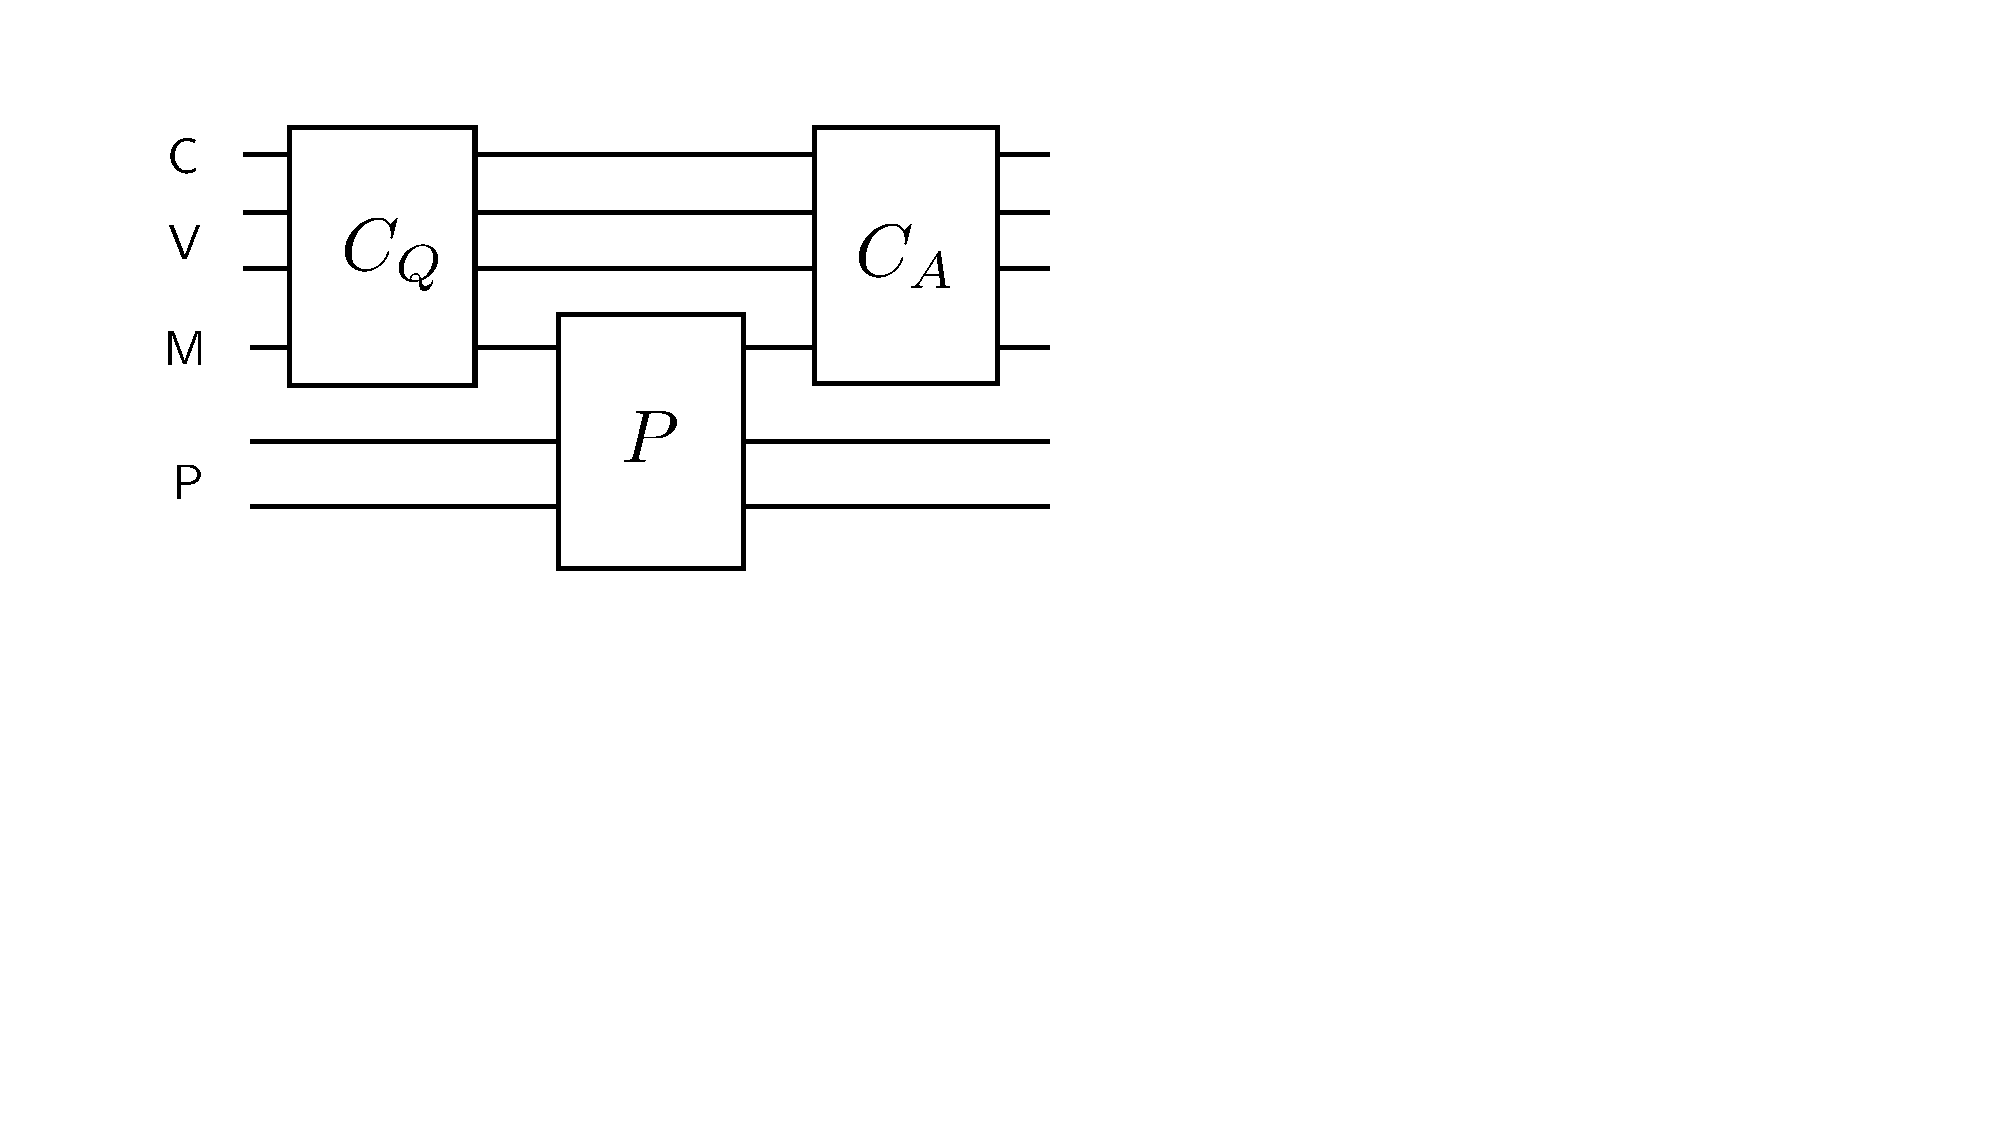
\includegraphics[width=4in]{graphics/qip3.pdf}
\end{center}
\caption{Three-turn quantum interactive protocol circuit.}
\label{fig:qip}
\end{figure}

A verifier $V = (C_Q,C_A)$ will implicitly define $3$-turn quantum interactive protocol for some number of provers. We will\tnote{we will --- when??} let $\Protocol_V$ denote this protocol.



\subsubsection{Non-local games} 

\tnote{moved this section here}

An $r$-player \textbf{non-local game} is a special kind of interactive protocol, where there are only two turns (the first turn is omitted), and the message registers are classical. A non-local game $G$ is specified by a tuple $(\mathcal{Q},\mathcal{A},\mu,V)$ where $\mathcal{Q} = \mathcal{Q}_1 \times \cdots \times \mathcal{Q}_r$ and $\mathcal{A} = \mathcal{A}_1 \times \cdots \times \mathcal{A}_r$ are finite sets, $\mu$ is a distribution over $\mathcal{Q}$, and $V: \mathcal{Q} \times \mathcal{A} \to \{0,1\}$ is a predicate. 

%A non-local game is played in the following manner. Before the game starts, the players distribute a shared state $\rho_{\sP_1 \cdots \sP_r}$ between themselves where player $i$ gets register $\sP_i$. In the game, the referee uses private randomness to sample a tuple of \emph{questions} $\vec{q} = (q_1,\ldots,q_r)$ from $\mu$, and sends $q_i$ to player $i$, who then performs local measurements on register $\sP_i$ of $\rho$ and returns the measurement outcome $a_i \in \mathcal{A}_i$ (called an \emph{answer}) to the referee. The referee accepts if and only if $V(\vec{q},\vec{a}) = 1$, where $\vec{a} = (a_1,\ldots,a_r)$.

To formulate an $r$-player non-local game as a two-turn quantum interactive protocol we can introduce a circuit $C_Q$ that samples questions $(q_1,\ldots,q_r)$ from the distribution $\mu$, and saves a copy of $q_i$ in the register $\sM_i$. After the provers' unitaries $P = P_1 \otimes \cdots \otimes P_r$ have been applied, the circuit $C_A$ measures the registers $\sM$  in the standard basis to obtain a tuple of answers $(a_1,\ldots,a_r)$, and then computes the predicate $V((q_1,\ldots,q_r),(a_1,\ldots,a_r))$ to decide whether to accept or reject.




\subsubsection{Strategies}

Let $V = (C_Q,C_A)$ be a verifier for an $r$-prover protocol $\Protocol_V$. A \textbf{strategy} $\strat$ for $\Protocol_V$ consists of a pair $(\rho,\{P_i\}_{i\in\{1,\ldots,r\}})$, where
\begin{enumerate}
	\item $\rho$ is an entangled\tnote{why entangled? are the provers not allowed to use spearable states?} state on $r+1$ (finite dimensional) registers $\sC, \sP_1, \ldots, \sP_r$
	\item For each $i\in\{1,\ldots,r\}$, $P_i$ is a reflection acting on the \tnote{was: $\sM_i \sP_i$ registers}registers $\sM_i \sP_i$.
\end{enumerate}
Note that given $V$, the size of the register $\sC$ is fixed (because it is specified by the verifier circuit $V$) in any strategy $\strat$ for $\Protocol_V$. However, the size of the registers $\sP_i$, $i\in\{1,\ldots,r\}$, can be arbitrary.

The \textbf{value of $\strat$ in $\Protocol_V$} is denoted by $\omega^*_\strat(V)$ and is defined as
\[
	\omega^*_{\strat}(V) := \Tr \Paren{ \Pi_{out} \, \paren{ C_A P C_Q} \, \rho \otimes \ketbra{0}{0}_{\sV \sM} \, \paren{C_A P C_Q}^\dagger}
\]
where $\Pi_{out} = \ketbra{1}{1}_{\sV_{out}}$ is the projector onto the $\ket{1}$ state of the output qubit of the $\sV$ register, $\ketbra{0}{0}_{\sV \sM}$ is the all zeroes state in the $\sV \sM$ registers, and $P = P_1 \otimes \cdots \otimes P_r$. 


The \textbf{value of a protocol $\Protocol_V$} is denoted by $\omega^*(V)$ and is defined as 
\[
	\omega^*(V) := \sup_{\strat} \omega^*_\strat(V)
\]
where the supremum is over all (finite dimensional) strategies $\strat$ for $\Protocol_V$. 

%We can now describe the execution of this interactive protocol as a sequence of gates $G_1,G_2,\ldots,G_\tau$ corresponding to the sequence of Hadamard and Toffoli gates of the verifier circuits interleaved with the prover's unitaries $W_i$. In other words, the gate sequence $\{G_t\}$ consists entirely of Hadamard and Toffoli gates except for the prover's unitaries. %Note that $\tau = \poly(n)$ since the interactive protocol runs in polynomial time.


\subsubsection{Closeness of strategies} 

We define notions of closeness of strategies. 
%
%\begin{definition}[State-dependent closeness of POVMs]
%	Let $\rho \in \Dens(\sA)$ be a state and let $M = \{M^a\}_a,N = \{N^a\}_a$ be two POVMs that have the same set of possible outcomes. Then define 
%	\begin{align}
%		d_\rho \Paren{ M, N } := \Brac{ \sum_a \Norm{ M^a - N^a }_\rho^2 }^{1/2}.
%	\end{align}
%\end{definition}

\begin{definition}[Closeness of strategies]
	Let $V = (C_Q,C_A)$ be a verifier and let $\strat = (\rho,\{P_i\}), \strat' = (\rho',\paren{P_i'})$ be strategies for the $r$-prover protocol $\Protocol_V$. Then $\strat$ is \textbf{$\eps$-close} to $\strat'$ if and only if
	\begin{enumerate}
		\item $ \norm{ \rho - \rho'}_{tr} \leq \eps$
		\item $\Norm{ P \sigma P^\dagger - P' \sigma P'^\dagger }_{tr} \leq \eps$		
		%For all $i\in\{1,\ldots,r\}$, %for all $q \in \mathcal{Q}_i$,
		%\tnote{why this? the first condition says that having the second for $\rho$ or $\rho'$ is enough}
		
		%d_\rho(M_i(q),M_i'(q)) \leq \eps.
		%\Norm{ P - P' }^2_{\wt{\rho}} \leq \eps
		%\]
	\end{enumerate}
where \tnote{let's not use the notation :=, as it's hard to be systematic}$\sigma := C_Q \rho \otimes \ketbra{0}{0}_{\sV \sM} C_Q^\dagger$, $P = P_1 \otimes \cdots \otimes P_r$ and $P' = P_1' \otimes \cdots \otimes P_r'$.

\end{definition}

\begin{definition}[Isometric strategies]
	Let $\strat = (\rho,\{P_i\})$ and $\strat' = (\rho',\{P_i'\})$ be strategies for an $r$-prover protocol $\Protocol_V$ corresponding to some verifier $V = (C_Q,C_A)$, and $0\leq \eps\leq 1$. Suppose $\rho \in \Dens(\sC \sP_1 \cdots \sP_r)$ and $\rho' \in \Dens(\sC \sP_1' \cdots \sP_r')$. Then $\strat$ is \textbf{$\eps$-isometric} to $\strat'$ if and only if there exist isometries: $I_i : \sP_i \to \sP_i'$ for each $i\in\{1,\ldots,r\}$ such that the strategy $\wt{\strat} = (\wt{\rho}, \set{ \wt{P}_i })$ is $\eps$-close to $\strat'$, where $\wt{\strat}$ is defined by
	\begin{enumerate}
		\item $\wt{\rho} = (I_1 \otimes \cdots \otimes I_r) \rho (I_1 \otimes \cdots \otimes I_r)^\dagger$
		\item For all $i$, $\wt{P}_i = I_i P_i I_i^\dagger$.
	\end{enumerate}
\end{definition}


\begin{lemma}
\label{lem:close_strategies}
	Let $V = (C_Q,C_A)$ be a verifier and let $\strat_1 = (\rho_1,\{P^{(1)}_i\}),\strat_2= (\rho_2,\{P^{(2)}_i\})$ be strategies for $\Protocol_V$ such that $\strat_1$ is $\eps$-isometric to $\strat_2$. Then we have that\tnote{is a $^*$ missing in the $\omega$? Also in the proof}
	\[
		\Abs{ \omega_{\strat_1}(V) - \omega_{\strat_2}(V) } \leq 2\eps.
	\]
\end{lemma}
\begin{proof}
For notational convenience we omit the all zeroes state $\ketbra{0}{0}_{\sV \sM}$ in the calculations below. Let $\strat_3= (\rho_3,\{P^{(3)}_i\})$ be the strategy such that $\strat_1$ is \tnote{was: perfectly isometric; it's not defined}$0$-isometric to $\strat_3$ and $\strat_3$ is $\eps$-close to $\strat_2$. It is straightforward to verify that $\omega_{\strat_1}(V) = \omega_{\strat_3}(V)$. 
	
	Let $\strat_4 = (\rho_4,\set{ P^{(4)}_i})$ be such that $\rho_4 = \rho_2$ but $\set{P^{(4)}_i} = \set{P^{(3)}_i}$. Then
	\begin{align*}
		\abs{ \omega^*_{\strat_3}(V) - \omega^*_{\strat_4}(V)} &\leq \Abs{ \Tr\Paren{ (C_A P^{(3)} C_Q)^\dagger \Pi_{out} (C_A P^{(3)} C_Q) \paren{\rho_3 - \rho_2}} } \\
		&\leq \norm{ \rho_3 - \rho_2}_{tr} \\
		&\leq \eps\;,
	\end{align*}
	where $P^{(3)} = \bigotimes P^{(3)}_i$. The second inequality follows from matrix H\"{o}lder ($\Tr(AB) \leq \|A\|_\infty \|B\|_{tr}$\tnote{sometimes we use $\|\cdot\|_1$, sometimes $\|\cdot\|_{tr}$. Are they the same thing? Can we use $\|\cdot\|_1$ only?}) and the last inequality follows from the fact that $\strat_3$ is $\eps$-close to $\strat_2$.
	Next, we have
	\begin{align*}
		\abs{ \omega^*_{\strat_2}(V) - \omega^*_{\strat_4}(V)} &\leq \Abs{ \Tr\Paren{ \Pi_{out} \Paren{ (C_A P^{(2)} C_Q)\rho_2 (C_A P^{(2)} C_Q)^\dagger  - (C_A P^{(3)} C_Q) \rho_2 (C_A P^{(3)} C_Q)^\dagger  } }} \\
		&\leq \norm{ (P^{(2)} C_Q) \rho_2 (P^{(2)} C_Q)^\dagger - (P^{(3)} C_Q) \rho_2 (P^{(3)} C_Q)^\dagger}_{tr} \\
		&\leq \eps.
	\end{align*}	
	The first inequality follows from matrix H\"{o}lder and the second inequality follows again from the fact that $\strat_3$ is $\eps$-close to $\strat_2$. Putting everything together we obtain the desired conclusion.

\end{proof}










\subsection{Turing machines}
\label{sec:turing_machines}

\tnote{moved this here from the next section, as it sounds like ``preliminaries'' material}

An \textbf{oblivious Turing machine} is one where the movement of the heads is independent of the input.

\begin{theorem}[Pippenger, Fischer~\cite{pippenger1979relations}]\label{thm:pippenger}
Any $k$-tape Turing machine $M$ that runs in time $T$ can be simulated by a $k$-tape oblivious Turing machine that runs in time $\poly(T)$. Furthermore, the location of the $k$ tape heads at time $1 \leq t \leq T$ can be computed in $\poly \log T$ time.
\end{theorem}


\subsubsection{Simulation of oblivious Turing machines with a quantum circuit}

\begin{lemma}\label{lem:tmsim}
	For all $T$, for every $k$-tape oblivious Turing machine $M$, there exists a quantum circuit $TMSIM(M,T)$ of size $\poly(T)$ where
	\begin{enumerate}
		\item $TMSIM(M,T)$ acts on registers $\sM \sA_1 \ldots \sA_k$
		\item The output of the $\{\sA_j\}$ registers of $TMSIM(M,T)$, when run on input $\ket{0}_{\sM} \otimes \ket{x}_{\sA_1 \cdots \sA_k}$, will be equal to the contents of $M$'s tapes on input $x$ after $T$ steps.
	\end{enumerate}
	Furthermore, there exists a Turing machine $\text{TMSIM-DESC}$ that on input $(M,T,t)$ (where $t$ is written in binary), it will output the $t$'th gate of $TMSIM(M,T)$ in $\poly\log(T)$ time. 
\end{lemma}

\begin{proof}
	The architecture of the circuit $TMSIM(M,T)$ is the following: the registers $\sM$ will store the state of the Turing machine $M$, and $\{\sA_j\}$ represent the work tapes of $M$. Since $M$ is oblivious, the head movement patterns of $M$ are pre-determined. Without loss of generality, each tape head will alternate between sweeping left for $T$ steps and then right for $T$ steps, and the heads will be moved in sequence (i.e., the first tape's head will move first, then the second tape's head will move, and so on). 
	
	Each $\sA_j$ register is $O(T)$ qubits wide, representing the $T$ cells of tape $j$ that $M$ could possibly access. Each movement of the heads of $M$ will correspond to a layer in the circuit; the computation of the head transition function of $M$ will be computed in the $\sM$ registers, which connected via two-qubit gates to the corresponding locations in the $\sA_j$ registers. 
	
	Since the computation of the transition function is some constant that only depends on the description size of $M$, the number of gates in each layer is a constant. Thus the total gate complexity of this circuit is $O(T)$. Notice that the gate sequence of each layer is the same, except the gates that cross between $\sM$ and the $\{\sA_j\}$ registers will be different depending on which cells of the tapes are supposed to be read at that layer. 
	
	Thus it is clear that it only takes $\poly\log T$ time to compute any desired gate of the circuit $TMSIM(M,T)$.
\end{proof}

\subsection{Circuits}

Analogously to the circuit $TMSIM$ that simulates a Turing Machine, we require the notion of universal circuit $CKTSIM$ that simulates an arbitrary circuit. 

\begin{lemma}\label{lem:cktsim}
For every integer $n$ there is a classical (resp. quantum) circuit $CKTSIM$ of size $\poly(n)$ that operates on $2n$ bits and is such that for any input $(C,x)$ where $x\in\{0,1\}^n$ and $C$ is the description of a classical (resp. quantum) circuit operating on at most $n$ bits returns $C(x)$. 
\end{lemma}

\subsection{Complexity theory}

\begin{definition}[Nondeterministic iterated exponential time]
	Let $R$ be a positive integer. Then we define
	\[
		\NEXPR = \NTIME[\exp^R_2(n)]
	\]
\end{definition}
with $n$ being the input size. 

We now define a canonically complete language for $\NEXPR$. Define $\mathcal{L}_R$ to be the set of all instances $\langle M, 1^n \rangle$ such that $M$, when interpreted as a nondeterministic Turing Machine, accepts after $\exp^R_2(n)$ steps on a blank tape as input.

\begin{definition}[$\MIPstar$]
	A language $L$ is in $\MIPstar(m,r)_{f(n)}$ if there is a $m$-player, $r$-round quantum interactive proof for $L$ with completeness-soundness gap $f(n)$, where $n$ is the input size. We write $\MIPstar(m,r) = \MIPstar(m,r)_{1/\poly(n)}$.
\end{definition}





\section{Simulated communication games}

In this section we introduce a variant of three-turn protocols, called \textbf{simulated communication games} (or \textbf{simcom games} for short), where the verifier and provers do not explicitly exchange message registers. Instead, they use quantum teleportation to communicate. Furthermore, whereas in teleportation the sender transmits classical teleportation keys to the receiver, in simcom games no such transmission takes place. Instead, the communicating parties \emph{guess} what the correct teleportation keys are; if their guess is incorrect, the protocol accepts. If the guess is correct, then acceptance or rejection is determined by an output bit of the verifier. This explains why we call the communication \emph{simulated}; the parties can effectively transmit messages to each other when we post-select on the correct teleportation keys.

\tnote{cut this:?}
The benefit of using simcom games is that the actions of the verifier and the provers are disjoint: they act on separate registers. This will be very useful for us in our recursive compression result. There will be a quantitative loss in transforming normal quantum interactive protocols to simcom games, but this loss will small provided that the original message lengths were small. 

More precisely, an $r$-prover simcom game involves a verifier $V$, which 
%an $r$-partite question alphabet $\cQ = \cQ_1 \times \cdots \times \cQ_r$, and an $r$-partite answer alphabet $\cA = \cA_1 \times \cdots \times \cA_r$. 
is still specified by two circuits $(C_Q,C_V)$ acting on registers $\sC \sV \sM$, and $r$ provers. The circuits $C_Q, C_A$ act on registers $\sC \sV \sM$ as before. However, the execution of the game is different from that of Figure \ref{fig:qip}. There are a number of extra registers: $\sK_1,\sK_2,\sK_2'$ are registers that are each isomorphic to two copies of $\sM$ (i.e. their dimensions are $(\dim \sM)^2$). The $\sK_1 \sK_2$ registers are initialized in the all zeroes state. The $\sK_2'$ register can start off in an arbitrary state. $\sE_1,\sE_1',\sE_2,\sE_2'$ are registers that are each isomorphic to $\sM$. They are initialized in the state  $\ket{\Phi}_{\sE_{1} \sE_{1}'} \otimes \ket{\Phi}_{\sE_{2} \sE_{2}'}$, where $\ket{\Phi}_{\sE_j \sE_j'}$ denotes the maximally entangled state between $\sE_j$ and $\sE_j'$. The allocation of registers is as follows: the verifier holds registers $\sK_1 \sK_2 \sC \sV \sM \sE_1 \sE_2$, and the $i$-th prover holds registers $\sE_{1,i}' \sE_{2,i}' \sP_i \sK_{2,i}'$. 

\medskip
\noindent The sequence of unitaries run in the simcom game is as follows:
\begin{enumerate}
	\item The circuit $C_Q$ is applied to registers $\sC \sV \sM$
	\item A Bell measurement is applied to the registers $\sM \sE_1$, and the measurement outcome is saved in $\sK_1$
	\item The provers then act on $\sE_1' \sE_2' \sP \sK_2'$, where the $i$-th prover's reflection is applied on $\sE_{1,i}' \sE_{2,i}' \sP_i \sK_{2,i}'$
	\item Then $m$ Hadamard gates are applied to $\sK_2$, where $m = \log \dim \sK_2$. In other words, the $\sK_2$ register stores the uniform superposition over all bitstrings of length $m$
	\item A SWAP gate is applied between $\sE_2$ and $\sM$
	\item Controlled on $\sK_2$, Pauli corrections (such as one would do in a teleportation protocol) is applied to the $\sM$ register
	\item The circuit $C_A$ is applied to $\sC \sV \sM$.
\end{enumerate}

%After the circuit $C_Q$ is applied, the maximally entangled state $\ket{\Phi}_{\sE_1 \sE_1'}$ is used to teleport the verifier's outgoing message to the provers: there is a teleportation circuit $TP$ acting on $\sM \sE_1$, which performs a Bell measurement on $\sM \sE_1$ and stores the measurement outcome in $\sK_1$. 

%The provers then act on $\sE_1' \sE_2' \sP \sK_2'$, where the $i$-th prover acts on $\sE_{1,i}' \sE_{2,i}' \sP_i \sK_{2,i}'$. Next, a SWAP gate is applied between $\sE_2$ and $\sM$. Then, the circuit $C_A$ is applied to $\sC \sV \sM$. Finally, $m$ Hadamard gates are applied to $\sK_2$, where $m = \log \dim \sK_2$. In other words, the $\sK_2$ register stores the uniform superposition over all bitstrings of length $m$. 

%However, instead of letting the provers act on $\sM \sP$ as before, the protocol behaves as follows: there are five additional registers $\sE_{1} \sE_{1}' \sE_{2} \sE_{2}' \sK$. The $\sE_j$ and $\sE_j'$ registers are each isomorphic to $\sM$. The $\sK$ register is isomorphic to two copies of $\sM$. The $\sE_1 \sE_1' \sE_2 \sE_2'$ registers are initialized in the state $\ket{\Phi}_{\sE_{1} \sE_{1}'} \otimes \ket{\Phi}_{\sE_{2} \sE_{2}'}$, where $\ket{\Phi}_{\sE_j \sE_j'}$ denotes the maximally entangled state between $\sE_j$ and $\sE_j'$. The $\sK$ register is initialized to all zeroes.

%The maximally entangled state $\ket{\Phi}_{\sE_1 \sE_1'}$ is used to teleport the verifier's outgoing message to the provers; after the circuit $C_Q$, there is a teleportation circuit $TP$ acting on $\sV \sM \sE_1$, which performs a Bell measurement on $\sM \sE_1$ and stores the measurement outcome in $\sV$. The provers then act on $\sE_1' \sE_2' \sP \sK$, where the $i$-th prover acts on $\sE_{1,i}' \sE_{2,i}' \sP_i \sK_i$. 

%Then, a SWAP gate is applied between $\sE_2$ and $\sM$. Finally, the circuit $C_A$ is applied to $\sC \sV \sM$. In addition to the output qubit $\sV_{out}$, we identify additional sub-registers of $\sV$, denoted by $\sV_{tp1},\sV_{tp2}$. These two registers are each isomorphic to two copies of $\sM$.

%The first register $\sV_{tp1}$ is isomorphic to two copies of $\cM$. The second register $\sV_{tp2}$ is isomorphic to two copies of $\cA$. 

\noindent See Figure \ref{fig:simcom} for the circuit representation of a simcom game.

\begin{figure}[H]
\begin{center}
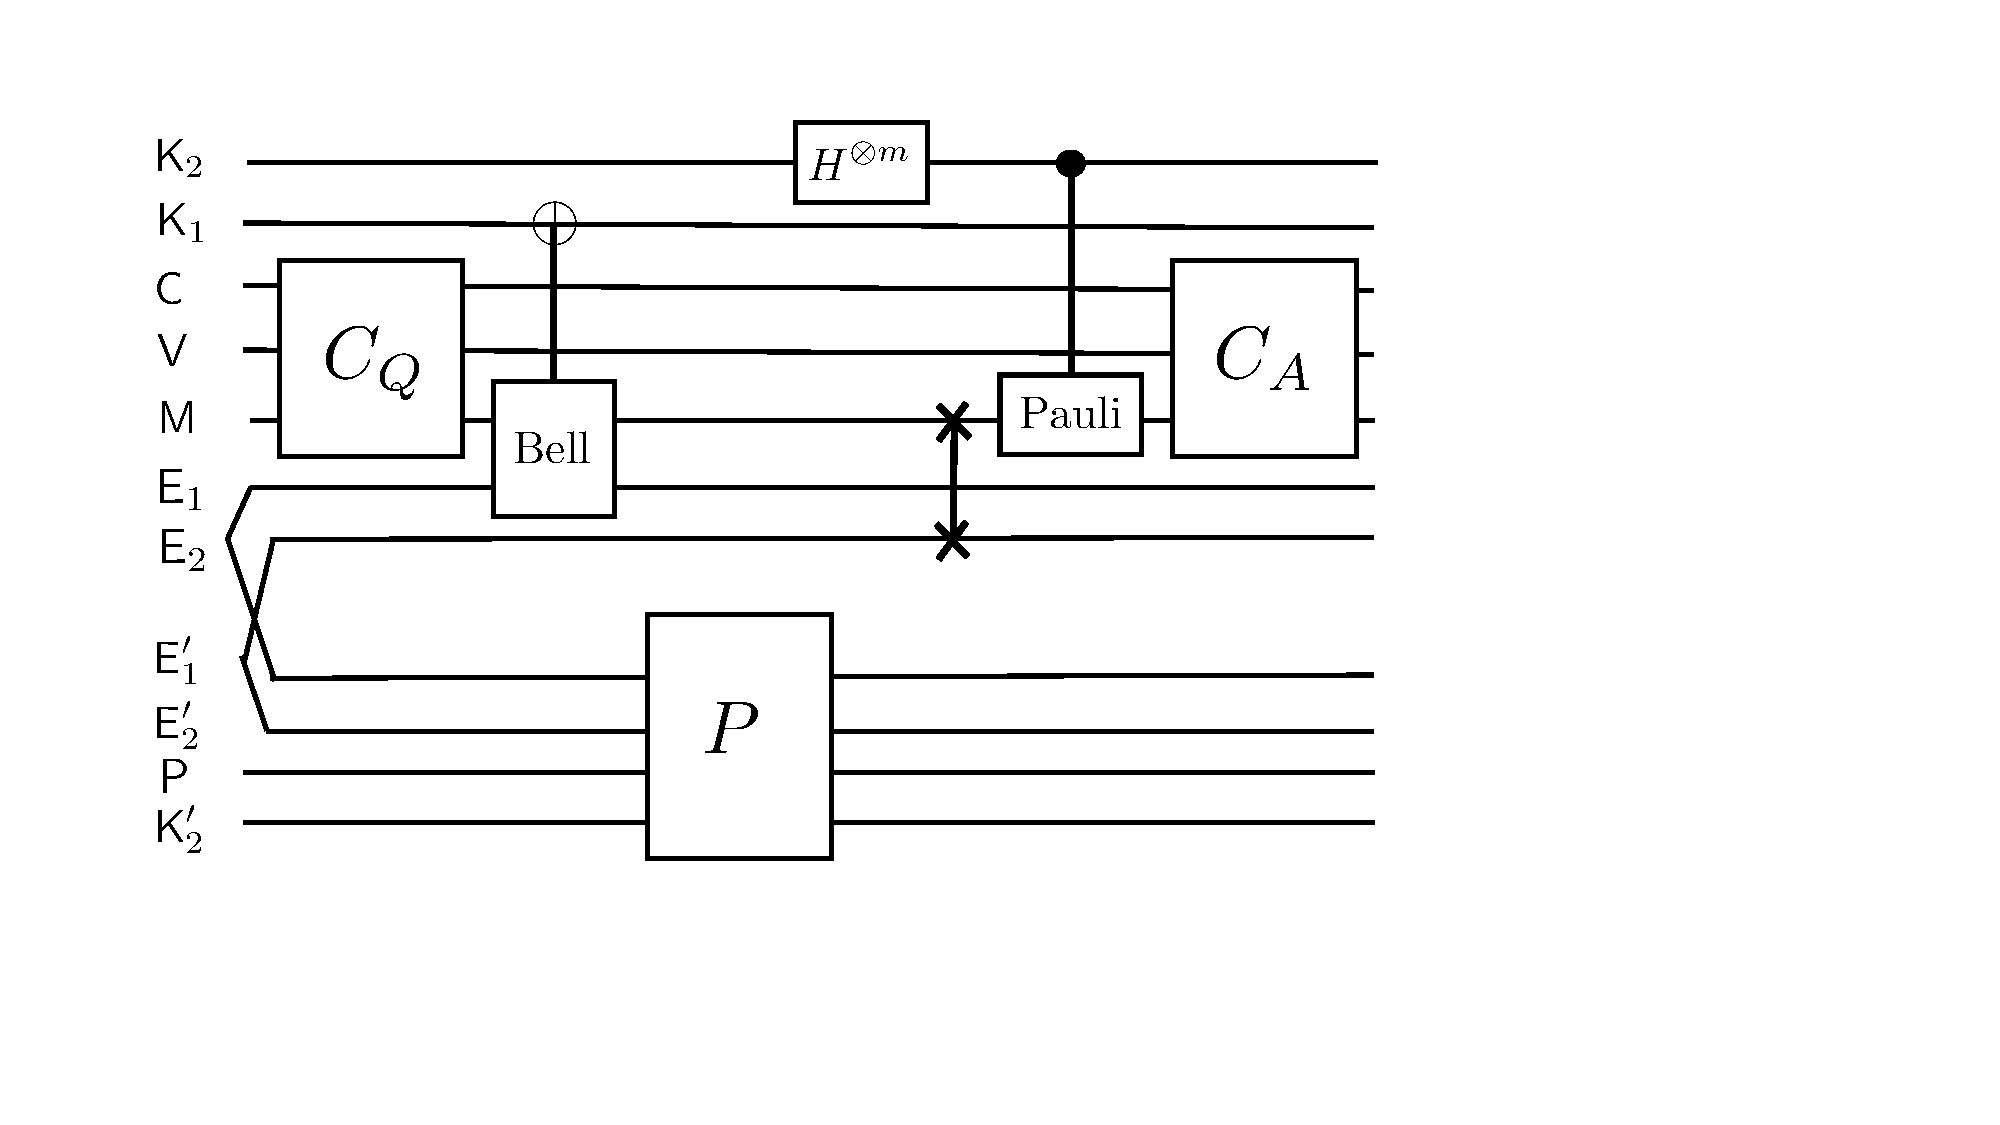
\includegraphics[width=4.5in]{graphics/simcom.pdf}
\end{center}
\caption{Simulated communication game circuit.}
\label{fig:simcom}
\end{figure}

Let $V = (C_Q,C_A)$ be a verifier and let $\mathscr{Z}_V$ denote the simcom game corresponding to $V$. We say that $V$ accepts in $\mathscr{Z}_V$ if measuring the $\sV_{out} \sK_1 \sK_2 \sK_2'$ registers yields outcome $(b,k_1,k_2,k_2')$ where $b = 1$, $k_1$ is all zero, and $k_2 = k_2'$. 

\paragraph{Strategies for simcom games} Strategies $\strat$ for simcom games are the similar to normal three-turn protocol strategies; they consist of a state $\rho$ and a collection of reflections $\{ P_i \}$. The shared state $\rho$ is on registers $\sC, \sP_1,\ldots,\sP_r$. The reflections $P_i$ act on registers $\sE_1' \sE_2' \sP_i \sK_{2,i}'$. Given a strategy $\strat = (\rho,\{P_i\})$, the \textbf{value of $\strat$ in $\mathscr{Z}_V$} is denoted by $\omega^{SC}(V)$ and is defined to be
\[
	\omega^{SC}_\strat(V) := \Tr \Paren{ \wt{\Pi}_{out} \, U \sigma U^\dagger}
\]
where
\begin{enumerate}
	\item $U =  (C_A) \,  (\text{C-Pauli}) \, (SWAP_{\sM \leftrightarrow \sE_2}) \, (H^{\otimes m}) \, (P)\, (\mathrm{Bell})\, (C_Q)$, where $\mathrm{Bell}$ is the Bell measurement circuit that saves the measurement outcome in register $\sK_1$ and $\text{C-Pauli}$ is the Pauli correction circuit that is controlled on $\sK_2$
	\item $\sigma = \rho \otimes \ketbra{0}{0}_{\sV \sM \sK_1 \sK_2 \sK_2'} \otimes \ketbra{\Phi}{\Phi}_{\sE_1 \sE_1'} \otimes \ketbra{\Phi}{\Phi}_{\sE_2 \sE_2'}$
	\item  $\wt{\Pi}_{out} = \ketbra{1}{1}_{\sV_{out}} \otimes \Pi_{tp} + (\Id - \Pi_{tp})$
	\item $\Pi_{tp} = \ketbra{0}{0}_{\sK_1} \otimes \Paren{ \sum_{k} \ketbra{kk}{kk}_{\sK_2 \sK_2'}}$.
\end{enumerate}
The unitary $U$ is the sequence of unitaries in the simcom game. The state $\sigma$ is simply $\rho$ along with the proper initialization for the protocol. The projector $\Pi_{tp}$ projects onto the state where $\sK_1$ is the zero state, and $\sK_2$ and $\sK_2'$ are equal when measured in the standard basis.

Finally, the \textbf{value of $\mathscr{Z}_V$} is denoted by $\omega^{SC}(V)$ and is defined to be the supremum of $\omega^{SC}_\strat(V)$ over all strategies $\strat$.


Although simcom games appear to be much more complicated than normal three-turn quantum interactive protocols, we emphasize that the verifiers for simcom games are exactly the same as in three-turn protocols; the only difference is in how the protocol is executed and how the value is defined. In the next lemma, we relate the value of a simcom game $\mathscr{Z}_V$ and the value of the three-turn protocol $\Protocol_V$ defined by $V$.

\begin{lemma}
\label{lem:convert_to_simcom}
	For all verifiers $V = (C_Q,C_A)$, $\omega^{SC}(V) = 1 - \frac{1 - \omega^*(V)}{\dim \sM^4}$. 
\end{lemma}
\begin{proof}
%	Let $V'$ behave as follows. The circuit $C_Q'$ is exactly the same as $C_Q$ (which we assume to act as the identity on the registers $\sV_{tp1} \sV_{tp2}$. The circuit $C_A'$ first initializes $\sV_{tp2}$ to be a uniformly random string, and then apply the Pauli correction operation on the $\sM$ register, assuming that the teleportation keys are given by $\sV_{tp2}$. Then it runs the circuit $C_A$. 
	We now argue that for every strategy $\strat$ for $\Protocol_V$, there is a strategy $\strat'$ for $\mathscr{Z}_V$ such that
	\begin{equation}
	\label{eq:simcom1}
		\omega^{SC}_{\strat'}(V) = 1 - \frac{1 - \omega^*_\strat(V)}{\dim \sM^4}.
	\end{equation}
	The strategy $\strat' = (\rho',\{P_i'\})$ is essentially the same as $\strat$: the states $\rho,\rho'$ are equal. The $i$-th prover $P_i'$ applies $P_i$ on $\sE_{1,i}' \sP_i$ (treating $\sE_{1,i}'$ as $\sM_i$). Then, it performs a Bell measurement on $\sE_{1,i}'$ and $\sE_{2,i}'$, saving the result of the Bell measurement in $\sK_{2,i}'$. In other words, the $i$-th prover uses $\sE_{1,i}'$ as its incoming message; it does not apply any Pauli corrections. Its message back to the verifier is teleported into the register $\sE_{2,i}'$. The probability that the keys $\sK_1$ from the first teleportation is equal to all zeroes is $(\dim \sM)^{-2}$. The probability the keys $\sK_2'$ from the second teleportation is equal to the verifier's guess in $\sK_2$ is also $(\dim \sM)^{-2}$. This establishes~\eqref{eq:simcom1}.
	
	This implies that $\omega^{SC}(V) \geq 1 - \frac{1 - \omega^*(V)}{\dim \sM^4}$. Now we argue for all strategies $\strat'$ for $\mathscr{Z}_{V}$, there exists a strategy $\strat$ for $\Protocol_V$ such that Equation~\eqref{eq:simcom1} holds. Let $\strat' = (\rho',\{ P_i' \})$. Define $\strat = (\rho,\{P_i\})$ where
	\begin{enumerate}
		\item $\rho = \rho' \otimes \ketbra{\Phi}{\Phi}_{\sE_1 \sE_1'} \otimes \ketbra{\Phi}{\Phi}_{\sE_2 \sE_2'} \otimes \ketbra{0}{0}_{\sK_2'}$. 
		
		\item The $i$-th prover $P_i$ receives registers $\sM_i \sP_i \sE_{1,i}' \sE_{2,i}' \sK_{2,i}'$ in this strategy. It does the following: it teleports the register $\sM_i$ into $\sE_{1,i}'$, applying Pauli corrections as needed. Then, it applies $P_i'$ to registers $\sE_{1,i}' \sE_{2,i}' \sP_i \sK_{2,i}'$. Then, it applies the Pauli correction operation on $\sE_{2,i}'$, using $\sK_{2,i}'$ as the correction keys. Then, it swaps the $\sE_{2,i}'$ register with the $\sM_i$ register. 
	\end{enumerate}
	It is straightforward to verify that~\eqref{eq:simcom1} holds. \hnote{Double check this.} This implies that $\omega^{SC}(V) \leq 1 - \frac{1 - \omega^*(V)}{\dim \sM^4}$, this proving the lemma.
\end{proof}


\subsubsection{Three-turn protocols with classical communication}

\tnote{Is this section needed? It doesn't seem to be saying much?}

Here we discuss three-turn protocols with classical messages. What we mean by this is that, in generating the message for the prover in the circuit $C_Q$, the verifier will save a copy of the message in the computational basis in its workspace register $\sV$. The circuit $C_A$, when viewed as a unitary, is classically controlled on the message register $\sM$. In other words, 
\[
	C_Q = \sum_{a} \ketbra{a}{a} \otimes C_Q^a 
\]
where $a$ runs over the computational basis states of $\sM$ and $C_Q^a$ is a unitary on $\sC \sV$. Furthermore, we will assume such protocols are equipped with a question and answer alphabet $\cQ = \cQ_1 \times \cdots \times \cQ_r$ and $\cA = \cA_1 \times \cdots \times \cA_r$, where the $i$-th prover receives questions from $\cQ_i$ and answers from $\cA_i$. We call these protocols \textbf{classical message protocols}, and their associated verifiers \textbf{classical message verifiers}.

Nonlocal games are an example of such protocols. We will also generally consider simcom games with classical communication. 

Strategies for such protocols can be expressed in a different way. As defined above, a strategy for a three-turn quantum interactive protocol consists of a shared state $\rho$ and a collection of reflections $\{ P_i \}$, one for each prover. We call these strategies \textbf{unitary strategies}, because the provers' actions are unitaries.

When the communication is classical, we can instead think of a \textbf{measurement strategy} $\cM$ which consists of a shared state $\rho$ along with a collection of POVMs $\{M_i\}$, where each $M_i$ is a map from $\cQ \times \cA$ to positive semidefinite matrices acting on $\sP_i$ satisfying $\sum_{a \in \cA_i} M_i(q_i,a_i) = \Id_{\sP_i}$ for all $i$ and $q_i$. In the context of non-local games, this is the notion of strategy typically considered: when the $i$-th prover receives a question $q_i$, it measures the $\sP_i$ register of $\rho$ to get an answer $a_i$. 
%We call such a strategy a \textbf{measurement strategy}, to distinguish it from a unitary strategy. 

A measurement strategy $\cM = (\rho,\{M_i\})$ has a canonical unitary strategy associated with it.
Let $\rho$ be on registers $\sC \sP_1 \cdots \sP_r$. Define $\strat_\cM = (\rho_U,\{P_i\})$ where $\rho_U = \rho \otimes \Paren{ \bigotimes_i \ketbra{0}{0}_{\sM_i'}}$ where $\sM_i'$ is an ancilla register isomorphic to $\sM_i$ given to the $i$-th prover (in addition to register $\sP_i$), and $P_i$ is defined as follows:
\[
	P_i = SWAP_{\sM_i \leftrightarrow \sM_i'} \cdot U_i
\]
with
\[
	U_i = \sum_{q_i} \ketbra{q_i}{q_i}_{\sM} \otimes \sum_{a_i} M_i(q_i,a_i)_{\sP_i} \otimes \ketbra{a_i}{0}_{\sM_i'}.
\]
The unitary $U_i$ is nothing but the Stinespring dilation of the channel that measures $\sP_i$ using the POVM $M_i(q_i)$. It saves the measurement outcome in the register $\sM_i'$. The unitary $P_i$ then swaps the $\sM_i$ and $\sM_i'$ registers after first applying $U_i$. \footnote{Technically speaking, we need to make $P_i$ a reflection by adding an additional ancilla qubit, but to keep the presentation simple we omit this detail for now.} 

The value of a protocol $\Protocol_V$ with respect to a measurement strategy $\cM$, denoted by $\omega^*_{\cM}(V)$, is defined to be $\omega^*_{\strat_\cM}(V)$. We also define the value of a simcom protocol $\mathscr{Z}_V$ with respect to $\cM$ to be the same as the value of a $\mathscr{Z}_V$ with respect to $\strat_\cM$. 

We now argue that in a classical message protocol, every unitary strategy $\strat$ has an associated measurement strategy $\cM_\strat$ whose value is equal to the one under the unitary strategy.

\begin{lemma}
\label{lem:unitary_measurement_strat}
Let $V = (C_Q,C_A)$ be a classical message verifier. Then for all unitary strategies $\strat = (\rho,\{ P_i \})$ there exists a measurement strategies $\cM_\strat = (\rho_\cM,\{M_i\})$ such that
	\[
		\omega^*_{\strat}(V) = \omega^*_{\cM_\strat}(V).
	\]
	and
	\[
		\omega^{SC}_{\strat}(V) = \omega^{SC}_{\cM_\strat}(V).
	\]	
\end{lemma}
\begin{proof}
\hnote{Insert proof here.}
\end{proof}

This lemma shows that for classical message protocols we can deal with measurement strategies. Throughout this paper, since we deal solely with classical message protocols, we will only deal with measurement strategies.

Notions of close and isometric measurement strategies are derived from close and isometric unitaries strategies: two measurement strategies $\cM$ and $\cM'$ are $\eps$-close if $\strat_{\cM}$ and $\strat_{\cM'}$ are $\eps$-close. A measurement strategy $\cM$ is $\eps$-isometric to $\cM'$ if $\strat_{\cM}$ is $\eps$-isometric to $\strat_{\cM'}$.  \hnote{May need to fix or spell out more explicitly...}

